\section{Analysis tasks}
\label{sec:analysis-tasks}

In this section, we study a gamut of fundamental analysis tasks, namely function reconstruction
(Section~\ref{sec:rmse-optimized}), gradient computation (Section~\ref{sec:gradient}), Laplacian
computation (Section~\ref{sec:laplacian}), histogram computation (Section~\ref{sec:histogram}), and
isocontour extraction (Section~\ref{sec:isocontour}). For each task, we define an error metric $E$
(see Section~\ref{sec:data_dep_streams}) that is the basis for evaluating stream's performance.
Algorithm~\ref{alg:greedy} is used to compute a greedy stream optimized separately for each task, in
terms of minimizing the relevant $E$ at every point. Each analysis task potentially requires a
fundamentally different stream for optimal results. Therefore, the goal is to distill the core
characteristics of these optimized streams. To accomplish this goal, we define and make use of a
concept named \emph{stream signature} (Section~\ref{sec:stream-signature}). The signature of a
stream is a small matrix that encodes the stream's ``preferences'' in terms of
precision-versus-resolution tradeoffs. As such, the signature not only reveals the characteristics
of a stream, but can also be used in practice to ``steer'' streaming in a way that is optimized for
particular task.

\subsection{Function reconstruction}
\label{sec:rmse-optimized}

The most fundamental analysis task is that of reconstructing the function itself. The most common
error metric in this case is the root-mean-square error (RMSE). For each data set, we use
Algorithm~\ref{alg:greedy} to construct an \emph{rmse-optimized} stream, and plot this stream
together with the three static streams (Section~\ref{sec:terminologies}) in
Figure~\ref{fig:rmse-optimized}. We also include \emph{rmse signature} streams, computed from the
signatures of \emph{rmse-optimized}. Note, again, that all leading-zero chunks are removed before
plotting, to emulate the effect of entropy compression often done in practice. It can be observed
that the difference between \emph{by wavelet norm} and \emph{rmse-optimized} is negligible in most
cases. This result is expected, because \emph{by wavelet norm} and \emph{rmse-optimized} both order
the chunks according to their contribution to in the $L_2$ sense, with \emph{rmse-optimized} also
taking into account the actual values of the bits. This difference has little effect, because, as
leading zero bits are removed, the rest of the bits (of the wavelet coefficients) are known to be
distributed approximately uniformly among $0$ and $1$.

\begin{figure}[h]
  \centering
	\subcaptionbox{Boiler}{
  {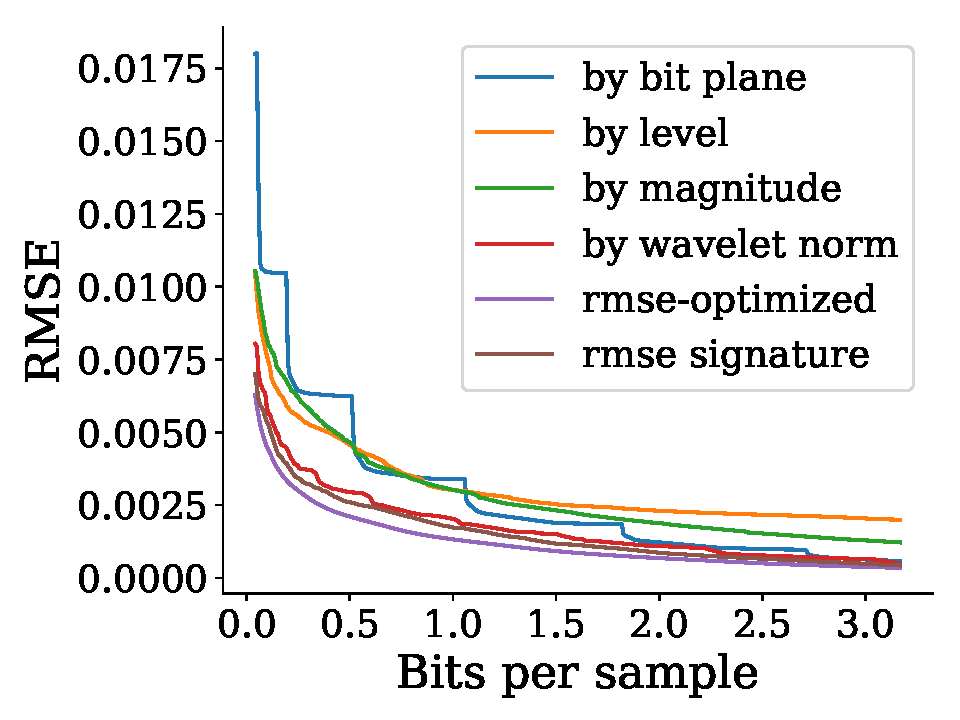
\includegraphics[width=0.48\linewidth]{rmse/rmse-optimized-boiler}}}
  \subcaptionbox{Diffusivity}{
  {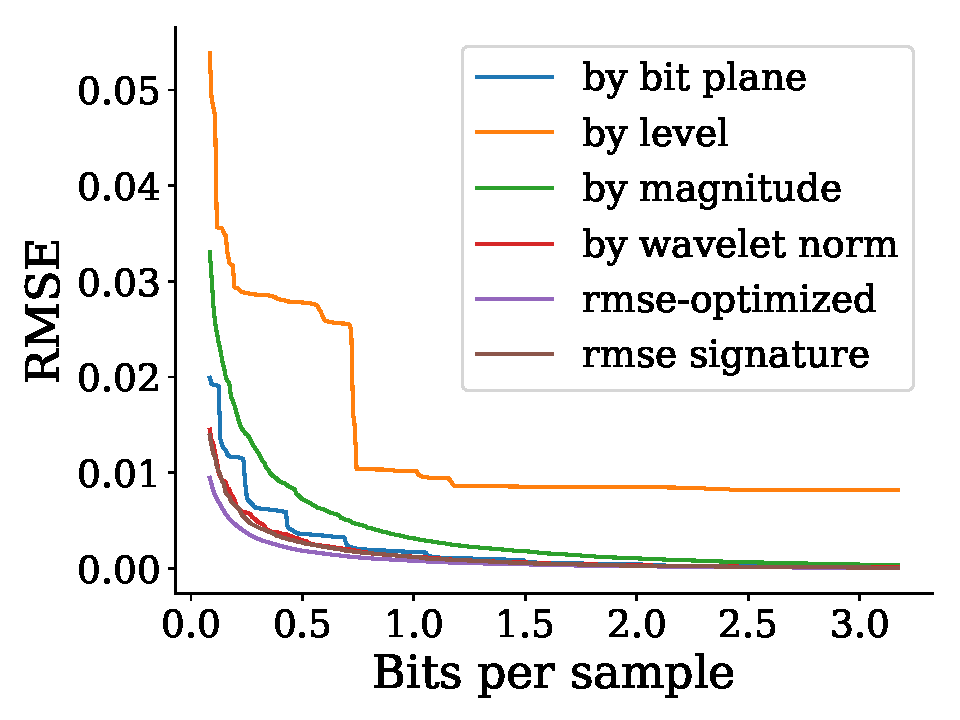
\includegraphics[width=0.48\linewidth]{rmse/rmse-optimized-diffusivity}}}
  \subcaptionbox{Plasma}{
  {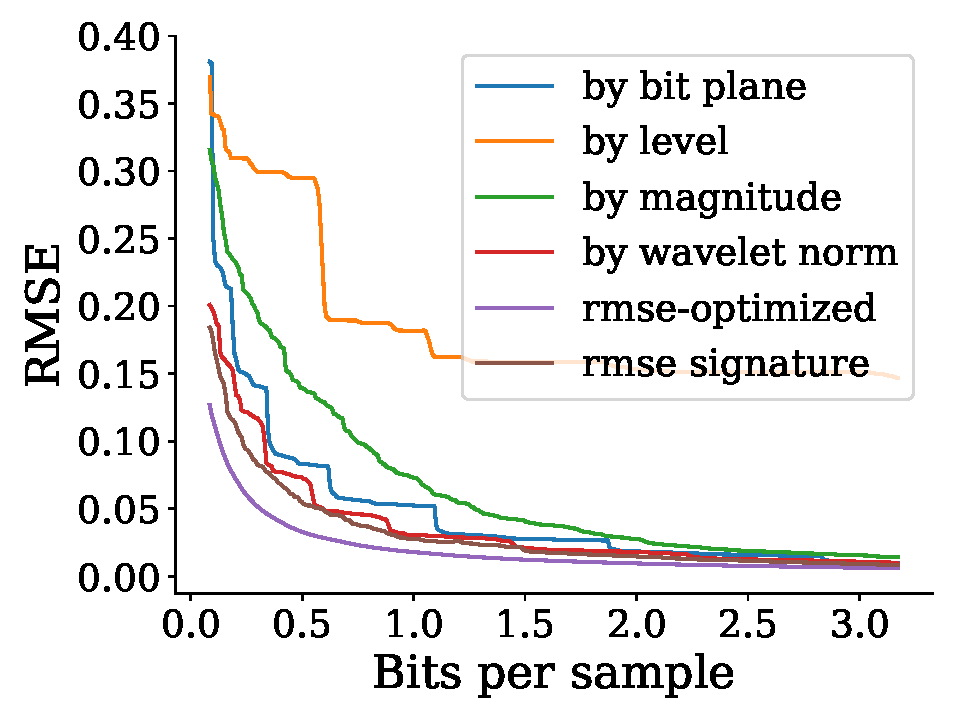
\includegraphics[width=0.48\linewidth]{rmse/rmse-optimized-plasma}}}
  \subcaptionbox{Turbulence}{
  {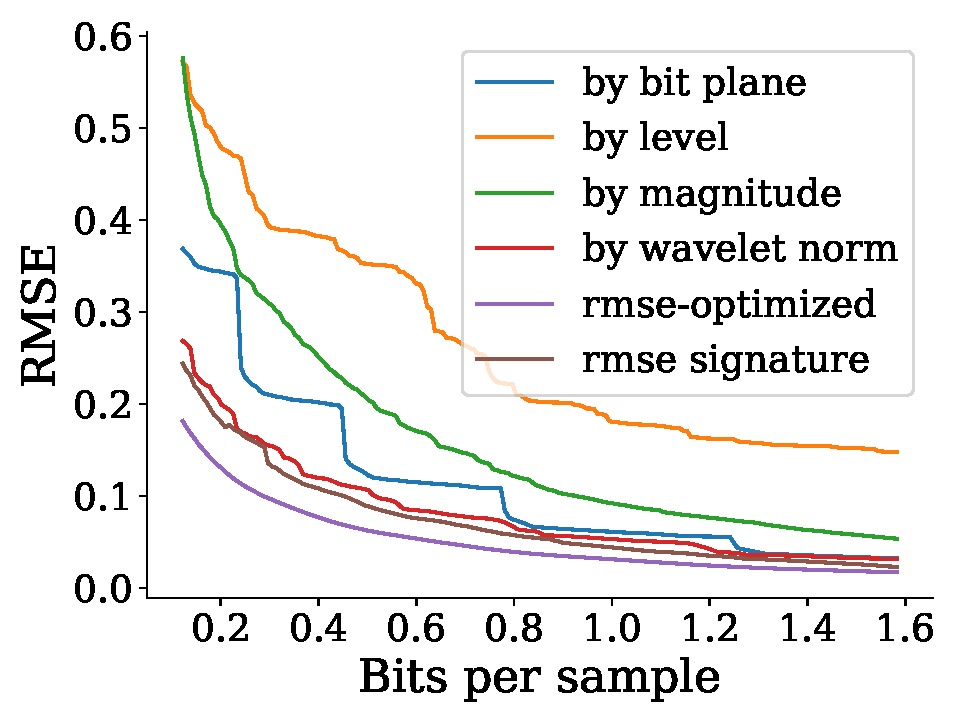
\includegraphics[width=0.48\linewidth]{rmse/rmse-optimized-turbulence}}}
  \caption{Root-mean-square error of reconstructed functions for the three data-agnostic streams
  defined in Section \ref{sec:motivation}, and the \emph{rmse-optimized} stream. Lower is better.
  The streams are truncated to highlight the differences, without omitting important information.
  \emph{rmse-optimized} performs best, followed closely by \emph{by wavelet norm}, \emph{rmse
  signature} and \emph{by bit plane}. TODO:explain any ``strange'' behavior in the plot.}
 	\label{fig:rmse-optimized}
\end{figure}

Among the static streams, \emph{by level} performs poorly compared to \emph{by bit plane}, \emph{by
wavelet norm}, and \emph{rmse signature}. This is because, in this case, low-ordered bits or
coarse-level coefficients contribute little compared to high-ordered bits of fine-level
coefficients. This difference in contribution is magnified when the data contains more fine-scale
features, as is the case for the \emph{plasma} data set. In Figure~\ref{fig:rmse-rendering}, we
render this field at 0.74 bits per sample (bps) for all three streams, and compare these rendering
with that of the groundtruth data. \emph{by level} results in heavy artifacts that are not seen by
\emph{by bit plane} and \emph{by wavelet norm}. \emph{by wavelet norm} performs slightly better than
\emph{by bit plane} here and in all other cases. In Figure~\ref{fig:precision-map-rmse}, it can be
observed that the distribution of bits per subband of the \emph{rmse signature} stream (and hence,
the \emph{rmse-optimized} stream) closely resembles that of \emph{by wavelet norm}. These results
suggest that in practice, \emph{by wavelet norm} is a near-optimal way to stream data that minimizes
root-mean-square errors, regardless of the data.

\begin{figure}[h]
	\centering
	\subcaptionbox{\emph{by level}}{
	{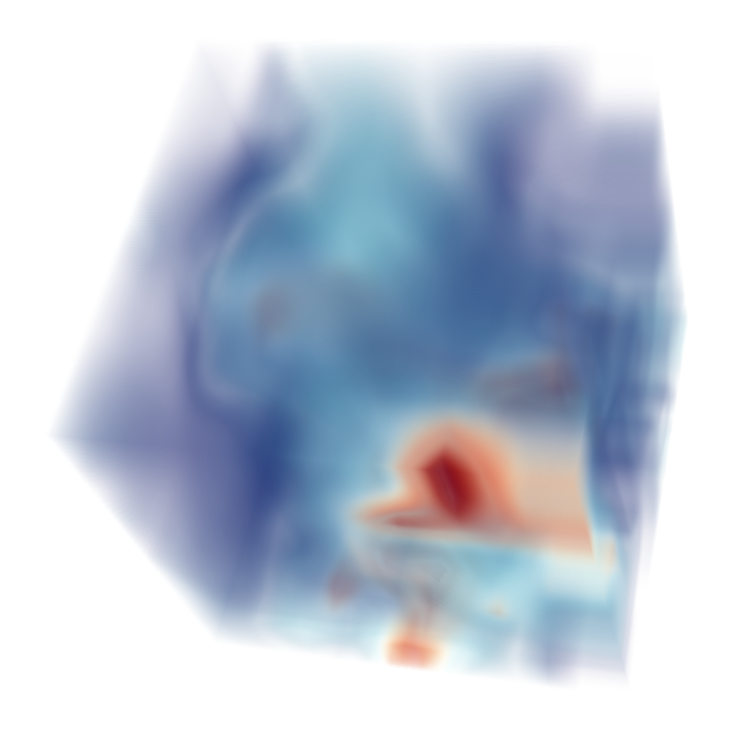
\includegraphics[width=0.31\linewidth]{rmse/rmse-boiler-level}}}
	\subcaptionbox{\emph{by bit plane}}{
	{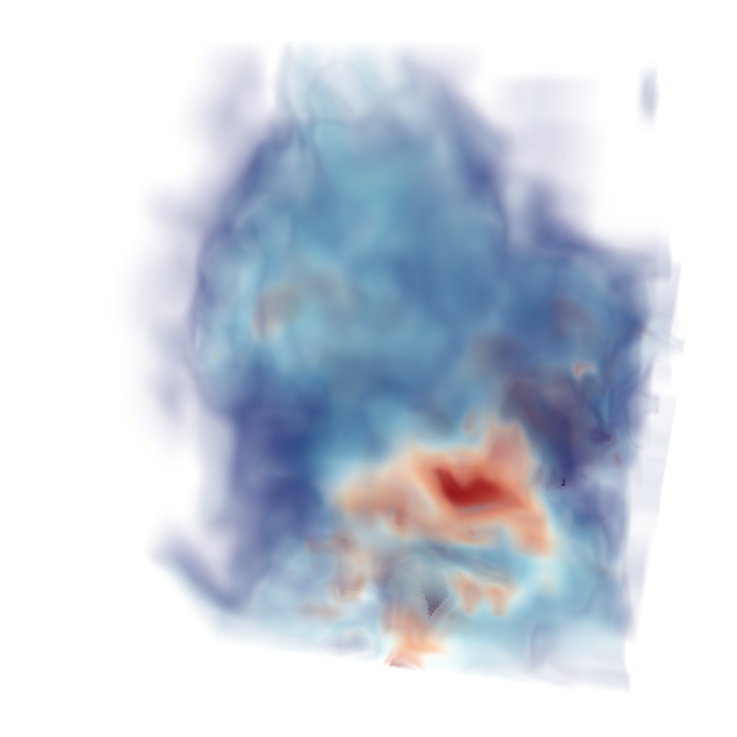
\includegraphics[width=0.31\linewidth]{rmse/rmse-boiler-bit-plane}}}
	\subcaptionbox{\emph{by magnitude}}{
	{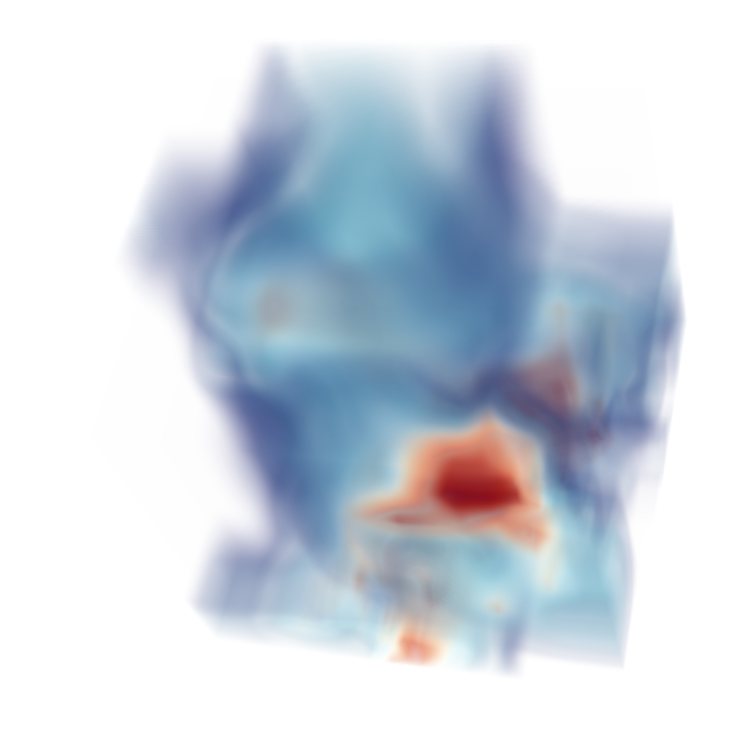
\includegraphics[width=0.31\linewidth]{rmse/rmse-boiler-magnitude}}}
	\subcaptionbox{\emph{by wavelet norm}}{
	{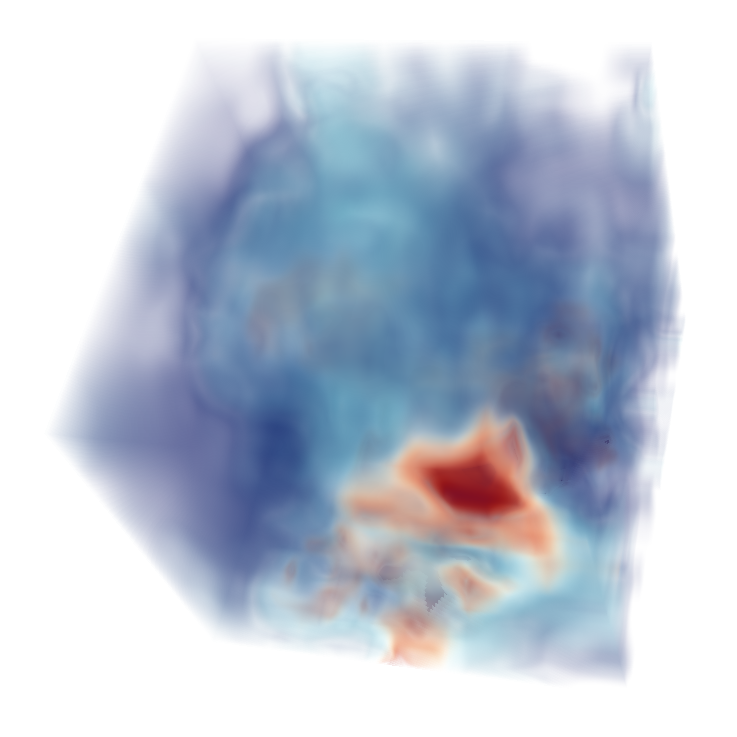
\includegraphics[width=0.31\linewidth]{rmse/rmse-boiler-wavelet-norm}}}
	\subcaptionbox{\emph{by signature}}{
	{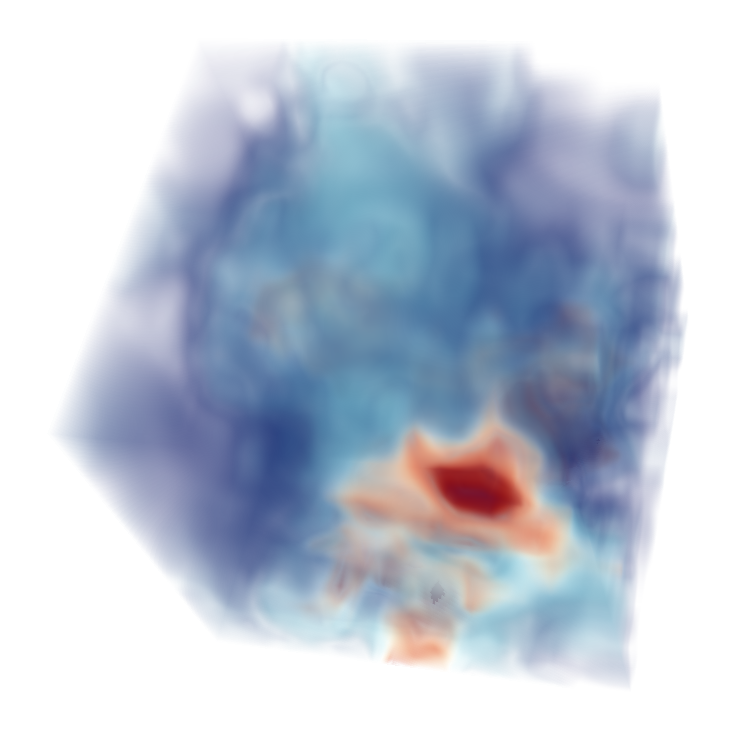
\includegraphics[width=0.31\linewidth]{rmse/rmse-boiler-signature}}}
	\subcaptionbox{\emph{groundtruth}}{
	{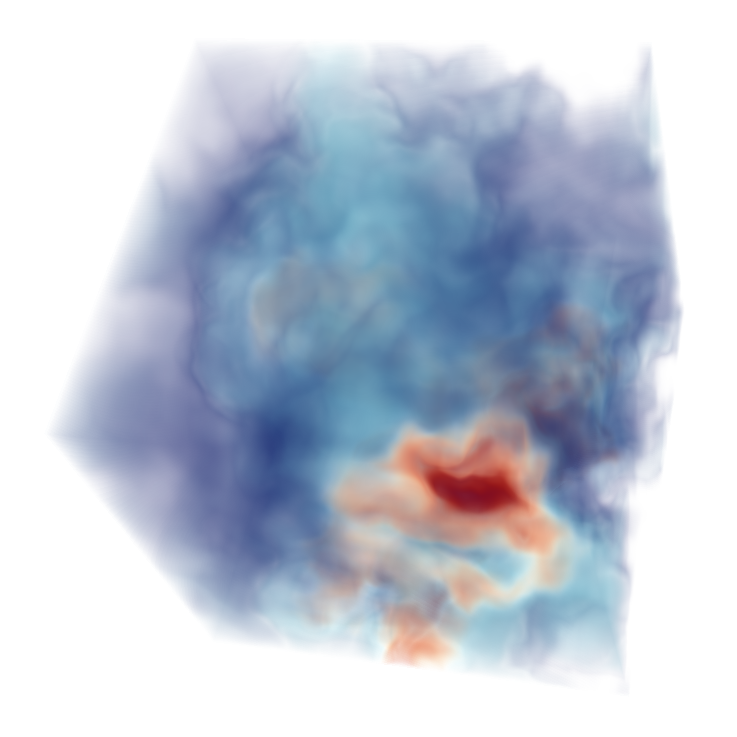
\includegraphics[width=0.31\linewidth]{rmse/rmse-boiler-groundtruth}}}
	\caption{\emph{boiler} data reconstructed at 0.03 bps}
 	\label{fig:rmse-rendering}
\end{figure}
